\documentclass{article}
\usepackage{amsmath}
\usepackage{graphicx}
\usepackage{listings}
\usepackage{xcolor}
\usepackage{hyperref}

\title{Lab 10}
\author{Rayane Guerou}

\begin{document}

\maketitle

\section{Introduction}
The Kuwahara filter is an image processing technique aimed at smoothing an image while preserving edges. It divides a region into four quadrants, selects the one with the lowest variance, and uses the mean color of that quadrant for the target pixel. We implemented the filter on the CPU, GPU, and GPU with shared memory to compare their performance.

\section{CPU Implementation of the Kuwahara Filter}
The CPU-based Kuwahara filter is applied using a nested loop for each pixel. The following function, \texttt{kuwahara\_region\_filter}, processes a subset of pixels in the local region.


The \texttt{apply\_kuwahara\_filter} function applies this filter to each pixel in the image. Below is the code for applying the filter.

\section{GPU Implementation of the Kuwahara Filter}
The GPU implementation uses CUDA to parallelize the processing of pixels. Each pixel is processed independently, allowing for faster execution.

The filter application is performed by calling the GPU function with specified CUDA grids and blocks.

\section{GPU Implementation with Shared Memory}
Using shared memory reduces global memory access by temporarily storing pixel values in fast local memory. This optimization improves performance for larger images.

\section{Performance Comparison}
To evaluate performance, we tested the three implementations with different \texttt{omega} values. Below are the results for each implementation, based on the neighborhood size.

\subsection{Performance Results}
\begin{itemize}
    \item \textbf{CPU:} Computation time increases proportionally with region size due to nested loops.
    \item \textbf{GPU:} Significant improvement with faster processing times, even for larger regions.
    \item \textbf{GPU with Shared Memory:} This is the fastest implementation, utilizing shared memory to minimize global access.
\end{itemize}


\section{CPU Result}
\begin{figure}[h!]
    \centering
    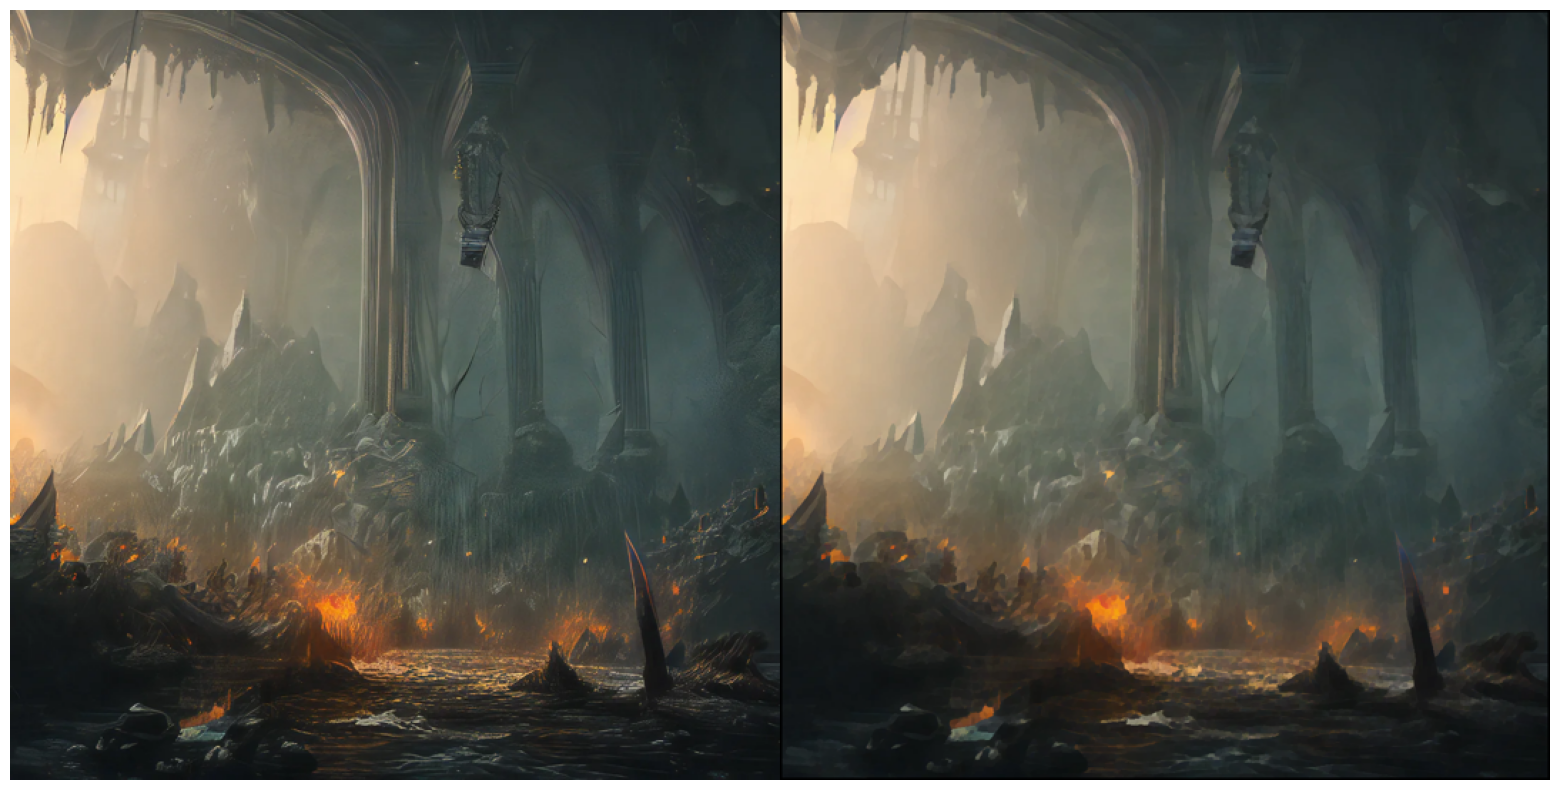
\includegraphics[width=0.5\textwidth]{src/cpu_result.png} 
    \caption{Output image using CPU implementation of the Kuwahara filter.}
\end{figure}

\section{GPU Result}
\begin{figure}[h!]
    \centering
    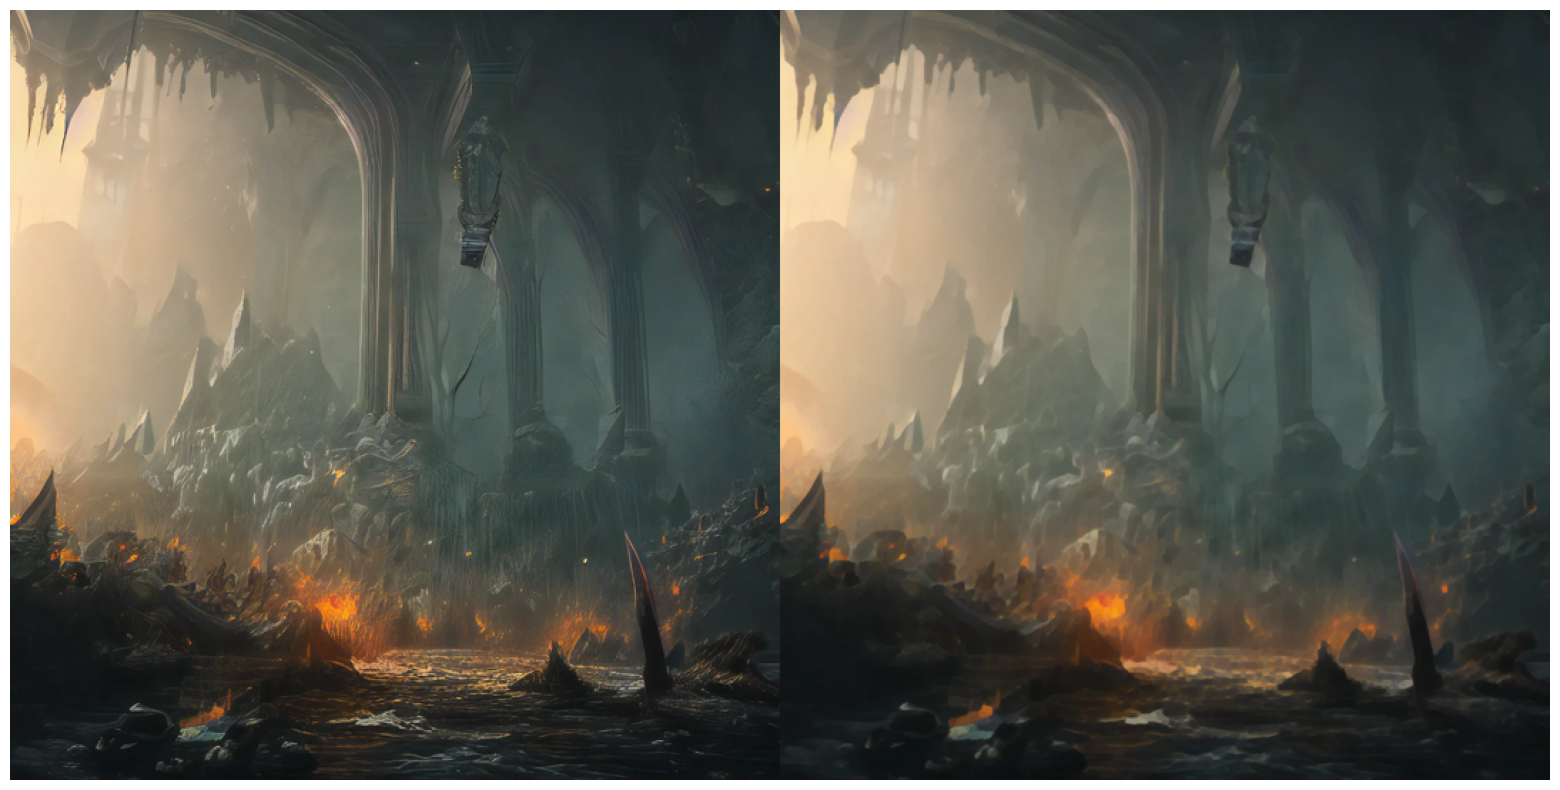
\includegraphics[width=0.5\textwidth]{src/gpu_result.png} 
    \caption{Output image using GPU implementation of the Kuwahara filter.}
\end{figure}

\section{GPU with Shared Memory Result}
\begin{figure}[h!]
    \centering
    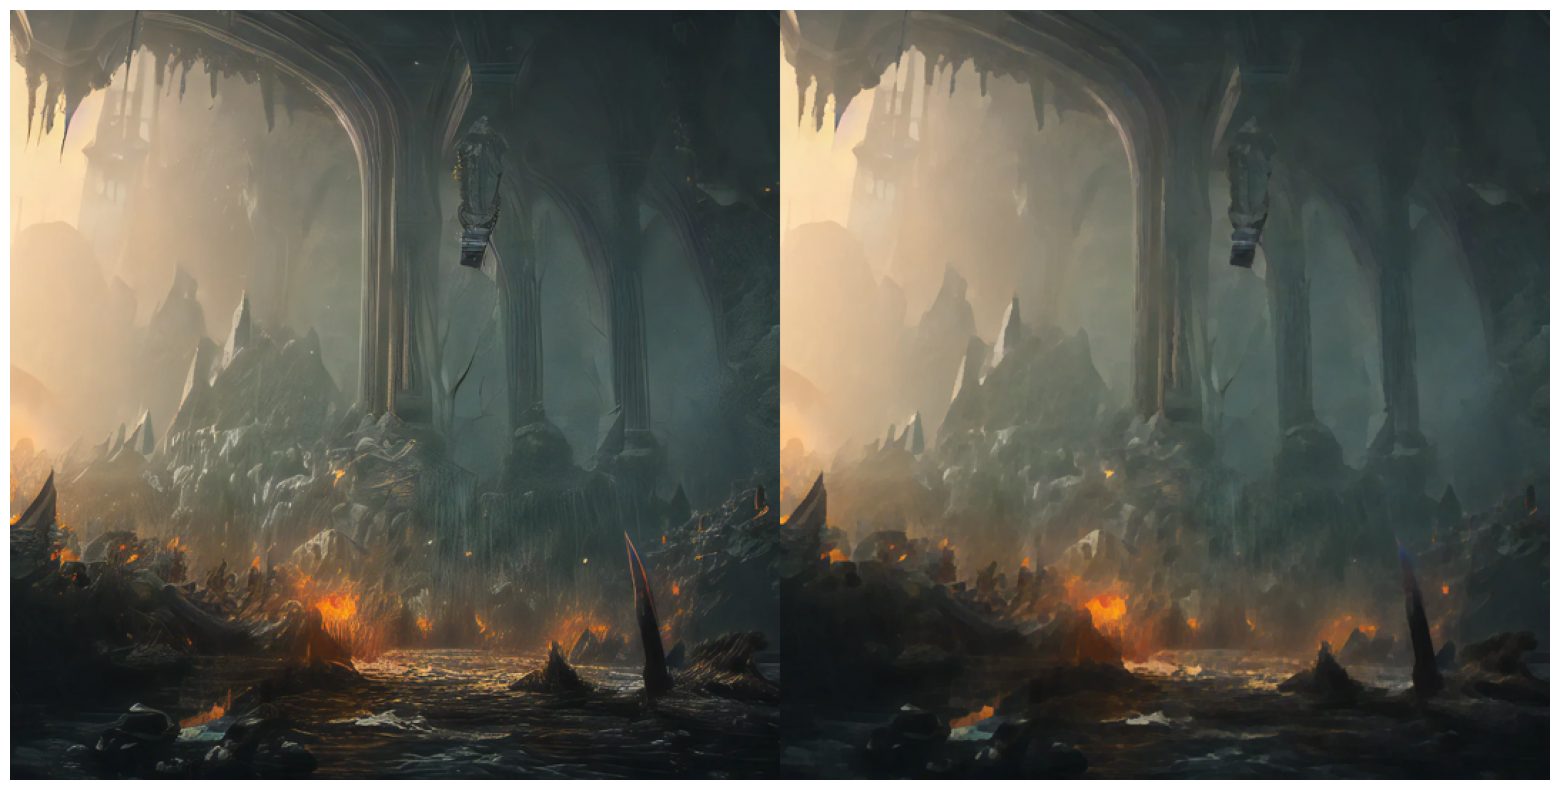
\includegraphics[width=0.5\textwidth]{src/gpu_shared_memory_result.png} 
    \caption{Output image using GPU with shared memory implementation of the Kuwahara filter.}
\end{figure}



\section{Conclusion}
We demonstrated how the Kuwahara filter can be optimized by leveraging GPU parallelism and shared memory. The results confirm that the GPU implementation with shared memory is the most efficient, particularly for large region sizes.

\end{document}